%\documentclass[12pt]{scrreprt}
\documentclass[12pt]{report} 

% language may be romanian or english (default is english)
% type may be bachelor or master (default is bachelor)
\usepackage[language=english, type=bachelor]{style}

%\geometry{a4paper,top=2.5cm,left=3cm,right=2.5cm,bottom=2.5cm}
%in style
%controlling the appearance of your headers and footers
\usepackage{fancyhdr}
\pagestyle{fancy}
\lhead{}
\chead{}
\renewcommand{\headrulewidth}{0.2pt}
\renewcommand{\footrulewidth}{0.2pt}

\usepackage{enumitem}

\usepackage[table]{xcolor} % https://www.overleaf.com/learn/latex/Tables#:~:text=its%20default%20height.-,Colour%20alternating%20rows,-You%20can%20apply
\usepackage{tabularx}


\begin{document}

\specialization{COMPUTER SCIENCE - ENGLISH}	
\title{Attractions}					   
\author{Pătrulescu Ronald Sandrino}											
\supervisor{Lect. dr. Pop Andreea Diana}				
				
\maketitle

% Why...?
\setbool{@eng}{false}
\specialization{INFORMATICĂ - ENGLEZĂ}
\title{Atracții}

\maketitle

% \newpage
% \thispagestyle{empty}
% \mbox{}
% \newpage
\pagenumbering{roman} 

\cleardoublepage
ABSTRACT
\vspace{0.5cm}	
\hrule
\vspace{0.5cm}	
%\cleardoublepage

\par With the increasing popularity of social media and the growing interest in travel, there is a need for innovative features in travel-related applications. This bachelor thesis presents the design and implementation of a web application that provides a platform that allows visualisation of attractions and the ability to create your own attractions or lists of such attractions.

\par The first chapter

\par The second chapter

\par The third chapter

\par The fourth chapter

\par The fifth and final chapter




\tableofcontents


\newpage
\pagenumbering{arabic}

\chapter{Introduction}

%\chapter*{Introducere}
\label{intro}

\par This chapter serves as an opening to the thesis, providing an overview of the motivation, background, objectives, and methodology behind the development of a travel-focused social media web application. While it builds on the abstract and preface by delving deeper into the subject, it also serves as a prelude to the technical and detailed discussions that will follow in subsequent chapters. The chapter is structured into several sections, each focusing on a particular aspect of the project.

\section{Motivation}

\par Travel, a cornerstone of shared experiences in the journey of life, serves as a dynamic conduit for the creation of enduring connections, precious memories, and deep personal insights. This potent medium invites us closer to each other, nature, and our inner selves, fostering a broader understanding of the world and our place within it. The exploration of diverse cultures and environments cultivates empathy and presents new perspectives, fulfilling the higher tiers of Maslow's hierarchy of needs such as self-actualization and transcendence. Living in a world driven fundamentally by relationships and the joy of experiencing the vitality of various cultures, travel becomes the nucleus of our most meaningful experiences. This basic human instinct to share individual journeys extends from the primal storytelling around a fire to the contemporary global narratives propelled by technology, underlining our collective yearning for shared experiences. Despite superficial differences, travel reveals profound commonalities between cultures, such as the instinct to survive, the pursuit of pleasure over pain, and our fundamental needs, thereby fostering empathy and reinforcing our interconnectedness.



\section{Background}

\par Numerous ground-breaking developments in computer science and technology have influenced the progress of web application development. In order to comprehend how the proposed travel-focused social media web application was developed, it is important to understand the key turning points that led to the current state of web apps. This section covers those turning points in detail.


\subsection{The Internet}

\par The invention of the internet fundamentally changed how people interact, obtain information, and conduct business in the modern day. The late 1960s and early 1970s saw the collaboration of numerous scholars and institutions to create the internet, often known as the "network of networks." The US Department of Defense's Advanced Research Projects Agency (ARPA) first created it as a decentralized communication network called ARPANET. Establishing a strong and resilient network that could endure partial failures and continue operating in the event of a calamity or military attack was the main driving force behind its design. The internet grew over time, connecting colleges, research centers, and eventually people all over the world. \cite{Cerf1974}

\subsection{The World Wide Web}

\par The World Wide Web (WWW), also referred to as the web, has transformed how we access and interact with information and has become a crucial part of the internet. While employed by the European Organization for Nuclear Research (CERN) in the late 1980s, Sir Tim Berners-Lee created the World Wide Web. His goal was to develop a system that would let users browse and distribute materials via hypertext links. WorldWideWeb, the first web browser, and the first web server were released in 1990 by Berners-Lee. These developments created the framework for the internet as we know it today. Fundamental web technologies like HTML (Hypertext Markup Language), which is used to structure web pages, and HTTP (Hypertext Transfer Protocol), which is used to communicate between servers and clients, allowed the web to grow quickly and be widely used. It changed the internet into a networked platform for dynamic content, multimedia, e-commerce, social networking, and many other applications from a collection of static documents. \cite{Berners1999}

\subsection{HTML}

\par As the common markup language for developing web pages and web applications, HTML (Hypertext Markup Language) is a vital component of the World Wide Web. It gives content, including as text, photos, multimedia components, and hyperlinks, a structure for organization and layout. The structure and display of web publications are defined by tags in HTML, which gives developers the ability to specify headings, paragraphs, lists, tables, forms, and other features. HTML's extensive popularity and function as the foundation of the web are due in part to its ease of use and adaptability. \cite{mozillaHTML}

\subsection{CSS and JavaScript}

\par The layout and formatting of HTML documents are described using the style-sheet language known as CSS (Cascading Style Sheets). It gives site designers control over elements like layout, colors, fonts, and animations that affect how online pages look. The structure of the web page is separated from the design elements using CSS, which makes it simpler to change and maintain the styling over several pages. With CSS, web designers can make websites that are visually appealing and responsive to various screen sizes and devices. \cite{mozillaCSS}

\par On the other hand, JavaScript is a flexible programming language that allows for dynamic behavior and interactivity on web sites. It enables programmers to handle events, create functionality, modify HTML components, and interact with servers. For producing interactive elements like form validation, sliders, carousels, and interactive maps, JavaScript is frequently utilized in web development. By providing real-time updates, client-side data processing, and seamless interaction with web apps, it improves the user experience. \cite{mozillaJS}

\subsection{AJAX}
\par Asynchronous JavaScript and XML (AJAX) is a set of web development tools that permits data to be exchanged asynchronously between a web browser and a server without requiring a page reload. To construct dynamic and interactive online applications, it mixes JavaScript, XML (or other data formats like JSON), and asynchronous communication. Because AJAX enables seamless data retrieval and display without interfering with the user's browsing experience, web developers may utilize it to construct responsive and interactive user interfaces. Jesse James Garrett is credited with popularizing AJAX in his seminal piece "Ajax: A New Approach to Web Applications," which appeared on the website of Adaptive Path in 2005. The article explored how AJAX, which enables more dynamic and responsive web applications, has the potential to transform web development. \cite{ajax}

\subsection{Emergence of Web Development Frameworks and Libraries}
\par Web development frameworks and libraries have emerged in recent years and have advanced quickly, altering how web applications are created. These frameworks and libraries give programmers a selection of instruments, pre-built frameworks, and reusable parts that speed up the programming process and increase productivity \cite{Seshadri2014}. They make it possible for developers to concentrate more on application logic than on low-level technical details, which makes it easier to create web apps that are reliable, scalable, and packed with features.

\par The introduction of these frameworks and libraries has greatly streamlined web development by enabling programmers to use pre-existing code, adhere to best practices, and follow established patterns. Routing, data binding, component-based architecture, form validation, and API connectivity are just a few of the many functionalities they provide \cite{Stefanov2021}. These technologies help developers create web apps more quickly and easily because they abstract complicated activities and offer well-documented APIs.

\par The ability of web development frameworks and libraries to address issues like code organization, code reusability, performance optimization, and cross-browser compatibility is a major factor in their success. Additionally, they encourage cooperation and knowledge exchange among developers through vibrant online communities, in-depth documentation, and a robust ecosystem of plugins and extensions.

\par Over time, a number of significant frameworks and libraries—including Angular, React, Vue.js, Django, Ruby on Rails, and Laravel—emerged, each with unique advantages and traits. These frameworks have a big impact on the web development scene and have been widely embraced by developers. \cite{vue} \cite{django} \cite{ruby} \cite{laravel}

\subsection{Evolution of Database Technologies}
\par Data management systems have become increasingly complex and effective as a result of tremendous evolution and innovation in the field of database technologies. This section examines the significant turning points in database technology development, highlighting noteworthy developments and their influence on the industry.

\begin{enumerate}
\item Hierarchical and Network Models
\par Network and hierarchical modeling were popular in the early days of database systems. Data was represented using these models, which were respectively pioneered by IBM's Information Management System (IMS) and the CODASYL Data Model, in the form of trees or graphs \cite{Date2003}. These models organized data well for the purposes of the applications they were designed for, but they lacked the adaptability to manage complicated relationships.

\item Relational Databases
\par Edgar Codd changed the database industry in the 1970s by introducing the relational model \cite{Codd1970}. In relational databases, data was arranged into tables with rows and columns and relationships defined by keys. Relational database management systems (RDBMS) based on SQL, such as Oracle, MySQL, and PostgreSQL, were made possible by this model's ability to store and query structured data in a powerful and flexible manner.

\item Object-Oriented Databases
\par As object-oriented programming languages became more popular, object-oriented databases (OODB) started to take the place of relational databases. By enabling the direct representation of objects in databases, OODBs sought to close the information storage and programming language gap \cite{Unland1990}. Complex data structures could be stored more easily as a result, and database models and application code were better integrated.

\item NoSQL Databases
\par NoSQL (Not Only SQL) databases were created as a result of the development of web applications and the necessity to manage massive amounts of unstructured and semi-structured data \cite{Hai2011}. NoSQL databases introduced flexible data structures such key-value, document, columnar, and graph databases in place of the classic relational databases' inflexible schema. These databases provide high availability, scalability, and effective management of various data kinds.

\item NewSQL Databases
\par The performance and scalability issues that traditional relational databases encountered in web-scale contexts led to the development of NewSQL databases \cite{Aslett2011}. These databases sought to combine the scalability and flexibility of NoSQL databases with the advantages of relational databases, such as ACID compliance. Improved performance, distributed architectures, and horizontal scalability were all features of NewSQL solutions.
\end{enumerate}

\subsection{Advances in Testing and Security}
\par Lorem \cite{}



\section{Objective and Scope}
\par The main goal of this thesis is to create and put into practice a social media web application that encourages users to connect with other travelers, discuss their travel experiences, and explore new places.

The entire development cycle—from initial system design and requirements analysis through functional implementation and testing—is covered by the thesis. It culminates in the integration and assessment of a customized trip recommendation system.

\section{Methodology}
\par The methodology for this project adopts an iterative approach to development, starting with a comprehensive requirements analysis and system design. Each component will be developed and tested individually, followed by integration and system-level testing. Continuous improvements and modifications will be made throughout the development process based on testing results.
%\addcontentsline{toc}{chapter}{Introducere}
%\addcontentsline{toc}{chapter}{Introduction}

\chapter{Theoretical frame}
\label{chap:ch1}

\section{REST}

\par lorem ipsmum
\chapter{Technical frame}
\label{chap:ch3}

\section{Backend}

\subsection{.NET and ASP.NET Core}

\par .NET (pronounced as "dot net") is a free, cross-platform, open-source developer platform for building many kinds of applications including web, desktop, mobile, cloud, IoT. It can run programs written in multiple languages, with C\# being the most popular. It relies on a high-performance runtime that is used in production by many high-scale apps. \cite{microsoftIntroDotNet} It was released in 2016 and its the successor of .NET Framework which dates way back to 2002.

\par ASP.NET Core is a free, cross-platform, open-source framework for building web apps and services with .NET and C\#. It is part of the app stack provided by .NET. Key features are: dependency injection, middleware pipeline, MVC, security.

\subsection{Entity Framework Core}

\par Entity Framework Core (EF Core) is an open source and cross-platform Object-Relational Mapping (ORM) framework for .NET applications. It is the successor to the original Entity Framework (EF) and has been redesigned to be lightweight and extensible. EF Core allows developers to work with a database using .NET objects, eliminating the need to write most of the data-access code manually. Key concepts:

\par \textbf{DbContext} is the primary class reponsible for interacting with the database. It manages the entity objects during runtime, tracks changes, handles the database interaction and allows customization of the ORM behavior.

\par \textbf{DbSet\textless{T}\textgreater{}} class represents a collection of entities of a specific type (`T`). Each DbSet in a DbContext corresponds to a table in the database and entity instance corresponds to a row in that table.

\begin{sloppypar} % in ordet to fix overflow
\par \textbf{Entities} are classes that map to tables in a relational database. Each property in an entity class corresponds to a column in the table (with certain exceptions, since EF allows defining a more complex behavior, as stated in  \url{https://learn.microsoft.com/en-us/ef/core/modeling/backing-field}) and each instance of the class corresponds to a row.
\end{sloppypar}


\par \textbf{LINQ (Language Integrated Query)} is used to query the database in a types-safe and object-oriented manner. It allows developers to write queries against the DbContext using standard C\# syntax:

\begin{figure}[!ht]
    \centering
    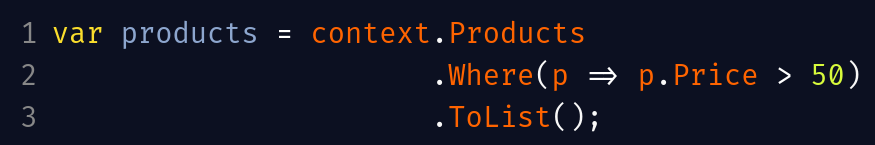
\includegraphics[width=1\linewidth]{linq-example.png}
\end{figure}

\par \textbf{Migrations} is a feature that helps managing database schema changes over the database's life-cycle. They allow you to incrementally apply changes to the schema, such as adding new tables, modifying columns, creating relationships between tables, etc, while preserving exitsting data.

\par \textbf{Change tracking}: EF Core automatically keeps track of changes made to entities during the lifetime of a DbContext instances. When \textit{SaveChanges()} is called, EF Core determines what changes have been made and generates the appropriate SQL commands to update the database.

\par \textbf{Relationships}: EF Core allows you to define relationships between entities, such as one-to-one, one-to-many, and many-to-many relationships. These relationships are represented using navigation properties and are enforced through foreign keys in the database.

\section{Frontend}

\subsection{React}

\par React is an open-source front-end JavaScript library released in 2013 by Meta (formerly Facebook). Back in 2011, the developers at Facebook started to face some issues with code maintenance. Which was caused by the increase in app features combined with cascading updates. The solution they arrived at is React. \cite{reactHistory} React does things by breaking down the UI into reusable components. This component-based architecture allows to build complex user interfaces by composing small, isolated pieces of code that manage their own state and logic. Key concepts:

\par \textbf{JSX} (\textbf{JavaScript XML}, formally \textbf{JavaScript Syntax eXtension}) is an XML-like extension to the JavaScript language syntax. \cite{jsx} It just a syntatic sugar that is transpiled into nested JavaScript function calls structurally similar to the original JSX. JSX lets you write HTML-like markup inside a JavaScript file. Inside React, it is used to define components.

\par \textbf{Components} are the UI building blocks in React. They are self-contained pieces of UI that can be reused throughout the application and are defined using JSX. They can be either functional (as the return of a function) or class-based (created by extending React.Component). Throughout the app, only functional components are used. Example of a functional component:

\begin{figure}[!ht]
    \centering
    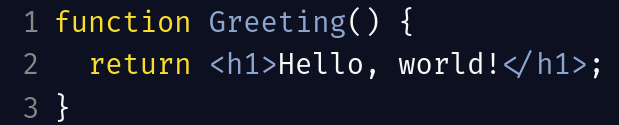
\includegraphics[width=1\linewidth]{react-component-example.png}
\end{figure}

\par \textbf{Props} (short for properties) are read-only data passed from a parent component to a child component. Props allow components to be dynamic and reusable by passing different data into them.

\par \textbf{Hooks} are function provided by the React API that provide features like "remembering" information like user input (useState), receiving information from a distant parent without passing it as props (useContext), holding information that isn't used for rendering (useRef), connecting to and synchronizing with external systems (useEffect). \cite{reactHooks}

\par \textbf{State} represents the internal writable data insides a component. State is declared using the \textbf{useState} hook which returns 2 the value of the state and a function to set that value. The value can be used directly in the JSX or to compute some other state. The setter should only be called inside other hooks or event handlers and not during rendering (i.e. directly inside functional components, which should be pure functions).

\par \textbf{Virtual DOM} In case of big pages, re-rendering can become an expensive operation. That's why react uses a virtual DOM, which is a copy of the real DOM. When the state of a component changes, a snapshot of its current virtual DOM is saved, then the virtual DOM is modified and compared with the snapshot and only then, the real DOM is changed based on the difference between the initial and the modified virtual DOM.

\subsection{TypeScript}

\par TypeScript is a strongly typed, compiled programming language that builds on JavaScript, one of the most widely used languages for web development. Developed and maintained by Microsoft, TypeScript introduces static typing to JavaScript, along with other features aimed at improving developer productivity and code maintainability. It has rapidly gained popularity in the web development community and is commonly used in conjunction with frameworks such as Angular, React, and Vue.js.

\par TypeScript is a superset of JavaScript, meaning any valid JavaScript code is also valid TypeScript code. TypeScript’s main feature is its optional static typing, which allows developers to define the types of variables, function parameters, and function return values. This helps catch errors at compile time rather than at runtime, leading to more robust and maintainable code.

\par TypeScript is transpiled into plain JavaScript, which can run in any environment that supports JavaScript, including web browsers, Node.js, and various JavaScript engines. The TypeScript compiler checks the code for type errors and compiles it into JavaScript that is compatible with the target environment.

\par TypeScript has type inference, which means the compiler can deduce the types of variables based on the values they are assigned. It also introduces interfaces, type aliases, access modifiers, generics and ES6 modules.

\par Using TypeScript comes with the advantage of strong typing, but the disadvantages are: the learning curve, the compilation step - converting the TypeScript code to JavaScript, which adds an extra layer of complexity to the development workflow and the dependency management.

\subsection{Redux}

\par Redux is an open-source JavaScript library for managing and centralizing application state. In React, centralized state management can be achieved to some degree using the \textit{useContext} feature. But, for medium to large-sized codebases with large amounts of application state and frequent and complex update logic, that might become too complex to maintain. Redux uses a single source of truth which contains read-only state that can only be modified through pure functions called reducers. The core components of Redux are the following:

\begin{itemize}
    \item Store - is the central object that holds the application’s state. It is created using the \textit{createStore} function provided by Redux. The store provides methods to access the state, dispatch actions, and subscribe to changes.
    \item State - is a single JavaScript object that represents the entire application’s data. It can only be updated by dispatching actions and processing those actions in reducers.
    \item Actions - are plain JavaScript objects that describe what happened in the application. Each action has a type property (a string constant) and can optionally have a payload property that carries additional data. Actions are dispatched to the store to trigger state changes.
    \item Reducers - are pure functions that take the current state and an action as inputs and return a new state. Reducers specify how the state should change in response to an action. Since reducers are pure functions, they do not modify the original state but return a new state object.
\end{itemize}

\par When a value in the state affects what is displayed to the user (example: the number of items in a shopping cart), that means that state defines the UI. When a user interacts with the page, by clicking a button or inputting text, an action is triggered (example: adding an item to the shopping cart). This action is dispatched to a reducer (example: the reducer receives an action of type addItemToCart with the payload being the id of the item). The reducers then updates the store (example: by adding the new item to the state that contains the shopping cart's items). And, since store contains the state, the changes are reflected everywhere the state is used (example: the count on the shopping cart increased by one and if you go to the checkout page, you will also see item you've just added). This can be seen in Figure \ref{fig:redux-flow}

\begin{figure}[!ht]
    \centering
    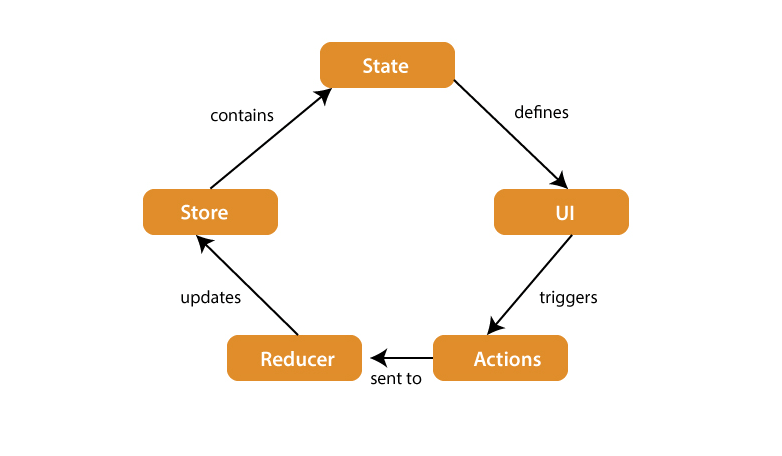
\includegraphics[width=1\linewidth]{redux-flow.png}
    \caption{Redux flow \cite{reduxFlow}}
    \label{fig:redux-flow}
\end{figure}

\subsection{Material UI}

\par Material UI (often abbreviated as MUI) is an open-source library that provides React components implementing Google's Material Design principles. Material Design is a design language developed by Google that emphasizes simplicity, consistency, and usability. Material-UI offers a comprehensive set of components and tools that help developers build aesthetically pleasing, responsive, and accessible user interfaces for web applications. Material UI provides various components like custom inputs, custom buttons, avatars, cards, dialogs, app bars, floating action buttons. Besides, it provides a powerful theming system that allows the customization of the appearance of components globally across the application, responsiveness through breakpoints and grids. It also includes a comprehensive set of Material Design icons that can be easily integrated into components. Icons are provided as React components and can be customized in terms of size, color, and other properties.

\begin{figure}[!ht]
    \centering
    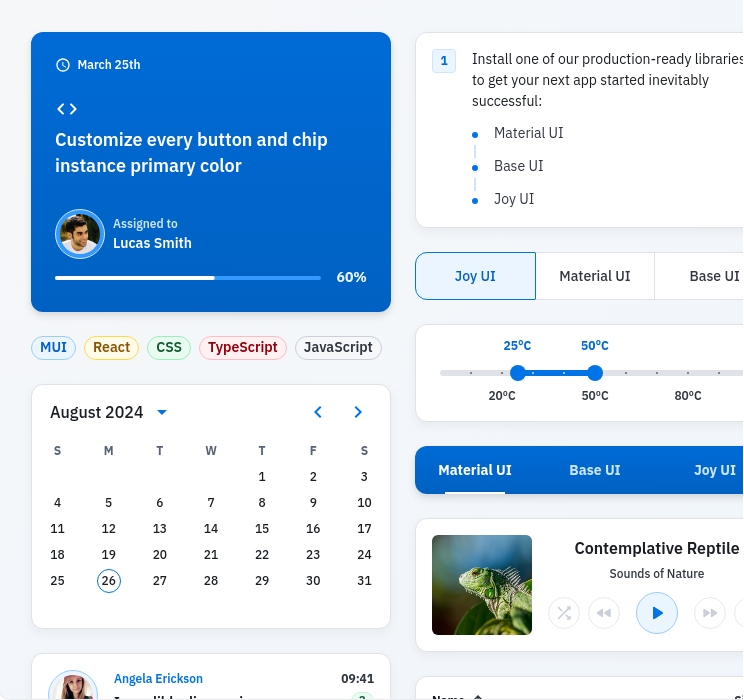
\includegraphics[width=1\linewidth]{material-ui-example.png}
    \caption{An example of what can be achieved with Material UI \cite{muiPreview}}
    \label{fig:enter-label}
\end{figure}
\chapter{Application}
\label{chap:ch4}

\section{Analysis}

\subsection{Functional requirements}

\par Throughout the application, the user can do the following:

\begin{itemize}
    \item Unauthenticated user
    \begin{itemize}
        \item Create an account
        \item Login into the application
        \item Reset their account's password
    \end{itemize}
    \item Regular user
    \begin{itemize}
        \item Log out of the application
        \item Change between light and dark theme
        \item Visualize, search, sort and filter attractions
        \item Add a new attraction or edit a created one
        \item React to an attraction with like or dislike
        \item Save an attraction to a new or existing collection
        \item Share an attraction to Threads, Twitter, Email or copy its link
        \item View an attraction's details on its page
        \item Comment on an attraction's page
        \item View their own and other users' profile
        \item Add or change their profile photo and description
        \item Send, accept and decline friend requests and unfriend current friends
        \item View their own and other users' friends
        \item View their own sent or received friend request
        \item View the list of their created attractions
        \item View the list of their collections
        \item Reorder their list of collections
        \item Add a new collection or edit/delete a created one
        \item View the details of a collection
        \item Reorder attractions within a collection
        \item Delete an attraction from the collection
        \item Set the picture of an attraction as the collection's picture.
    \end{itemize}
    \item Admin
    \begin{itemize}
        \item Anything a regular user can do
        \item View the list of attraction types and how many attractions are using them
        \item Add or rename attraction types
        \item Delete unused attraction types
    \end{itemize}
\end{itemize}


\subsection{Use cases}

\begin{figure}[!ht]
    \centering
    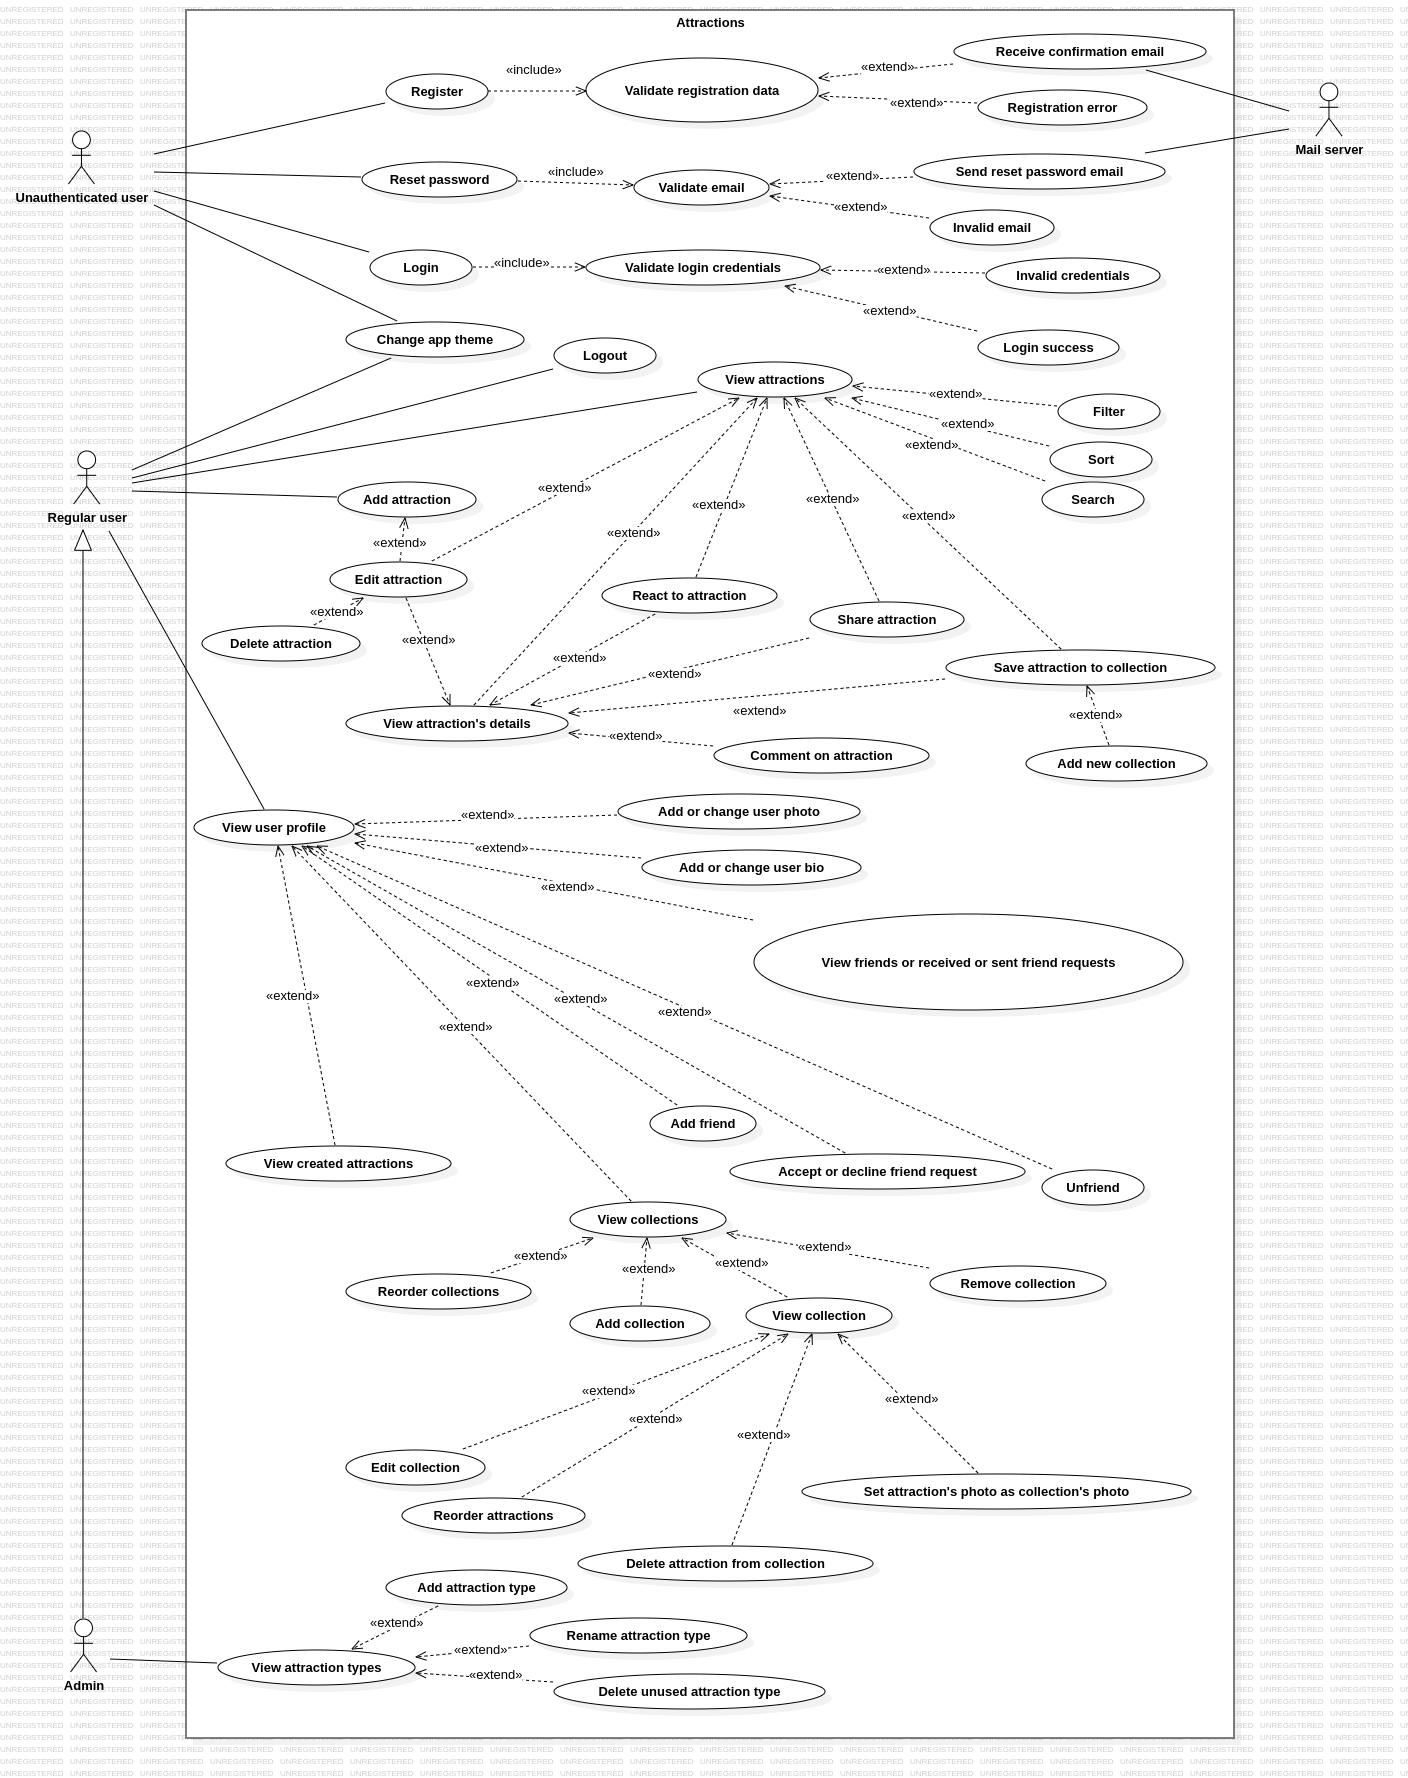
\includegraphics[width=1\linewidth]{UseCaseDiagram1.png}
    \caption{Use case diagram}
    \label{fig:enter-label}
\end{figure}

\clearpage % https://www.overleaf.com/learn/latex/Questions/How_can_I_get_my_table_or_figure_to_stay_where_they_are%2C_instead_of_going_to_the_next_page%3F

\begin{table}[!ht]
    \centering
    \begin{tabular}{|l|p{11cm}|}
        \hline
        \multicolumn{2}{|c|}{Use case: Register} \\
        \hline
         Actors & Regular User \\
        \hline
        Standard process & 
            % {\rowcolors{3}{green!20!yellow!50}{green!10!yellow!40}
            {\rowcolors{3}{gray!40}{gray!20}
                \begin{tabular}{|c|p{4.5cm}|p{4.5cm}|}
                    \multicolumn{3}{c}{} \\
                    \hline
                    No. & User action & System response \\
                    \hline
                    1 & User enters username, email and password then clicks the "Register" button & \\
                    \hline
                    2 &  & The systems validates the data, creates the account, sends the confirmation email and then displays a notification \\
                    \hline
                \end{tabular}
            } 
            \begin{tabular}{|c|p{4.5cm}|p{4.5cm}|}
                \multicolumn{3}{c}{} \\
            \end{tabular}
            \\
        \hline
         Alternative process & 
            {\rowcolors{3}{gray!40}{gray!20}
                \begin{tabular}{|c|p{4.5cm}|p{4.5cm}|}
                    \multicolumn{3}{c}{  } \\
                    \hline
                    No. & User action & System response \\
                    \hline
                    1 & User enters username, email and password then clicks the "Register" button & \\
                    \hline
                    2 &  & The systems validates the data, finds validation problems and shows the user the problems with each registration fieldd \\
                    \hline
                \end{tabular}
            } 
            \begin{tabular}{|c|p{4.5cm}|p{4.5cm}|}
                \multicolumn{3}{c}{} \\
            \end{tabular}
            \\
        \hline
         Preconditions & The user must be on the register page \\
        \hline
         Postconditons & If the registration is successful, the user will receive a confirmation email \\
        \hline
    \end{tabular}
\end{table}

\section{Architecture}

\par The application is structured on the client - server model. The client is a web application created using React and the server is a Web API created using the ASP.NET Core subset of the .NET Framework. For persistent storage the database used is SQLite. External services are used for email sending and photo upload.

\begin{figure}[!ht]
    \centering
    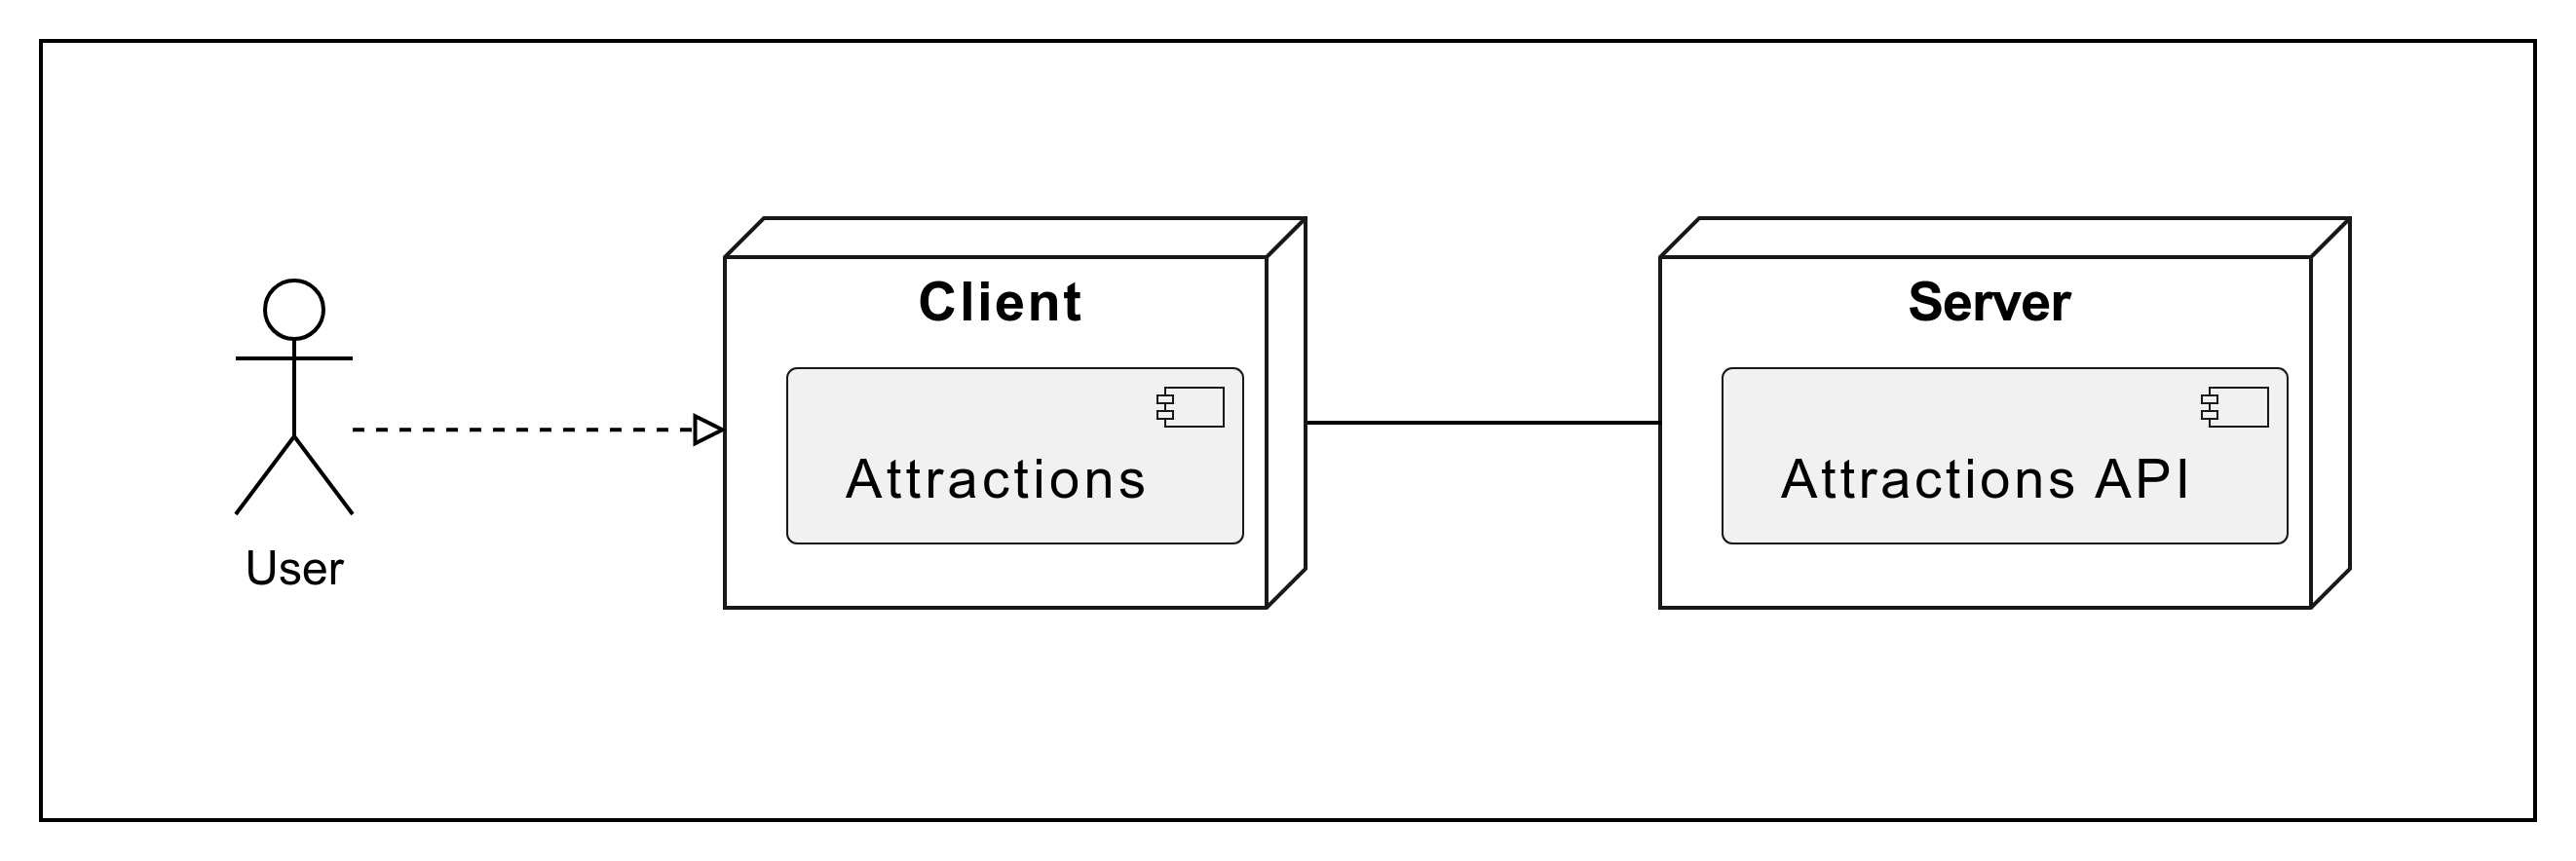
\includegraphics[width=1\linewidth]{app-architecture.png}
    \caption{Application architecture}
    \label{fig:enter-label}
\end{figure}

\begin{figure}[!ht]
    \centering
    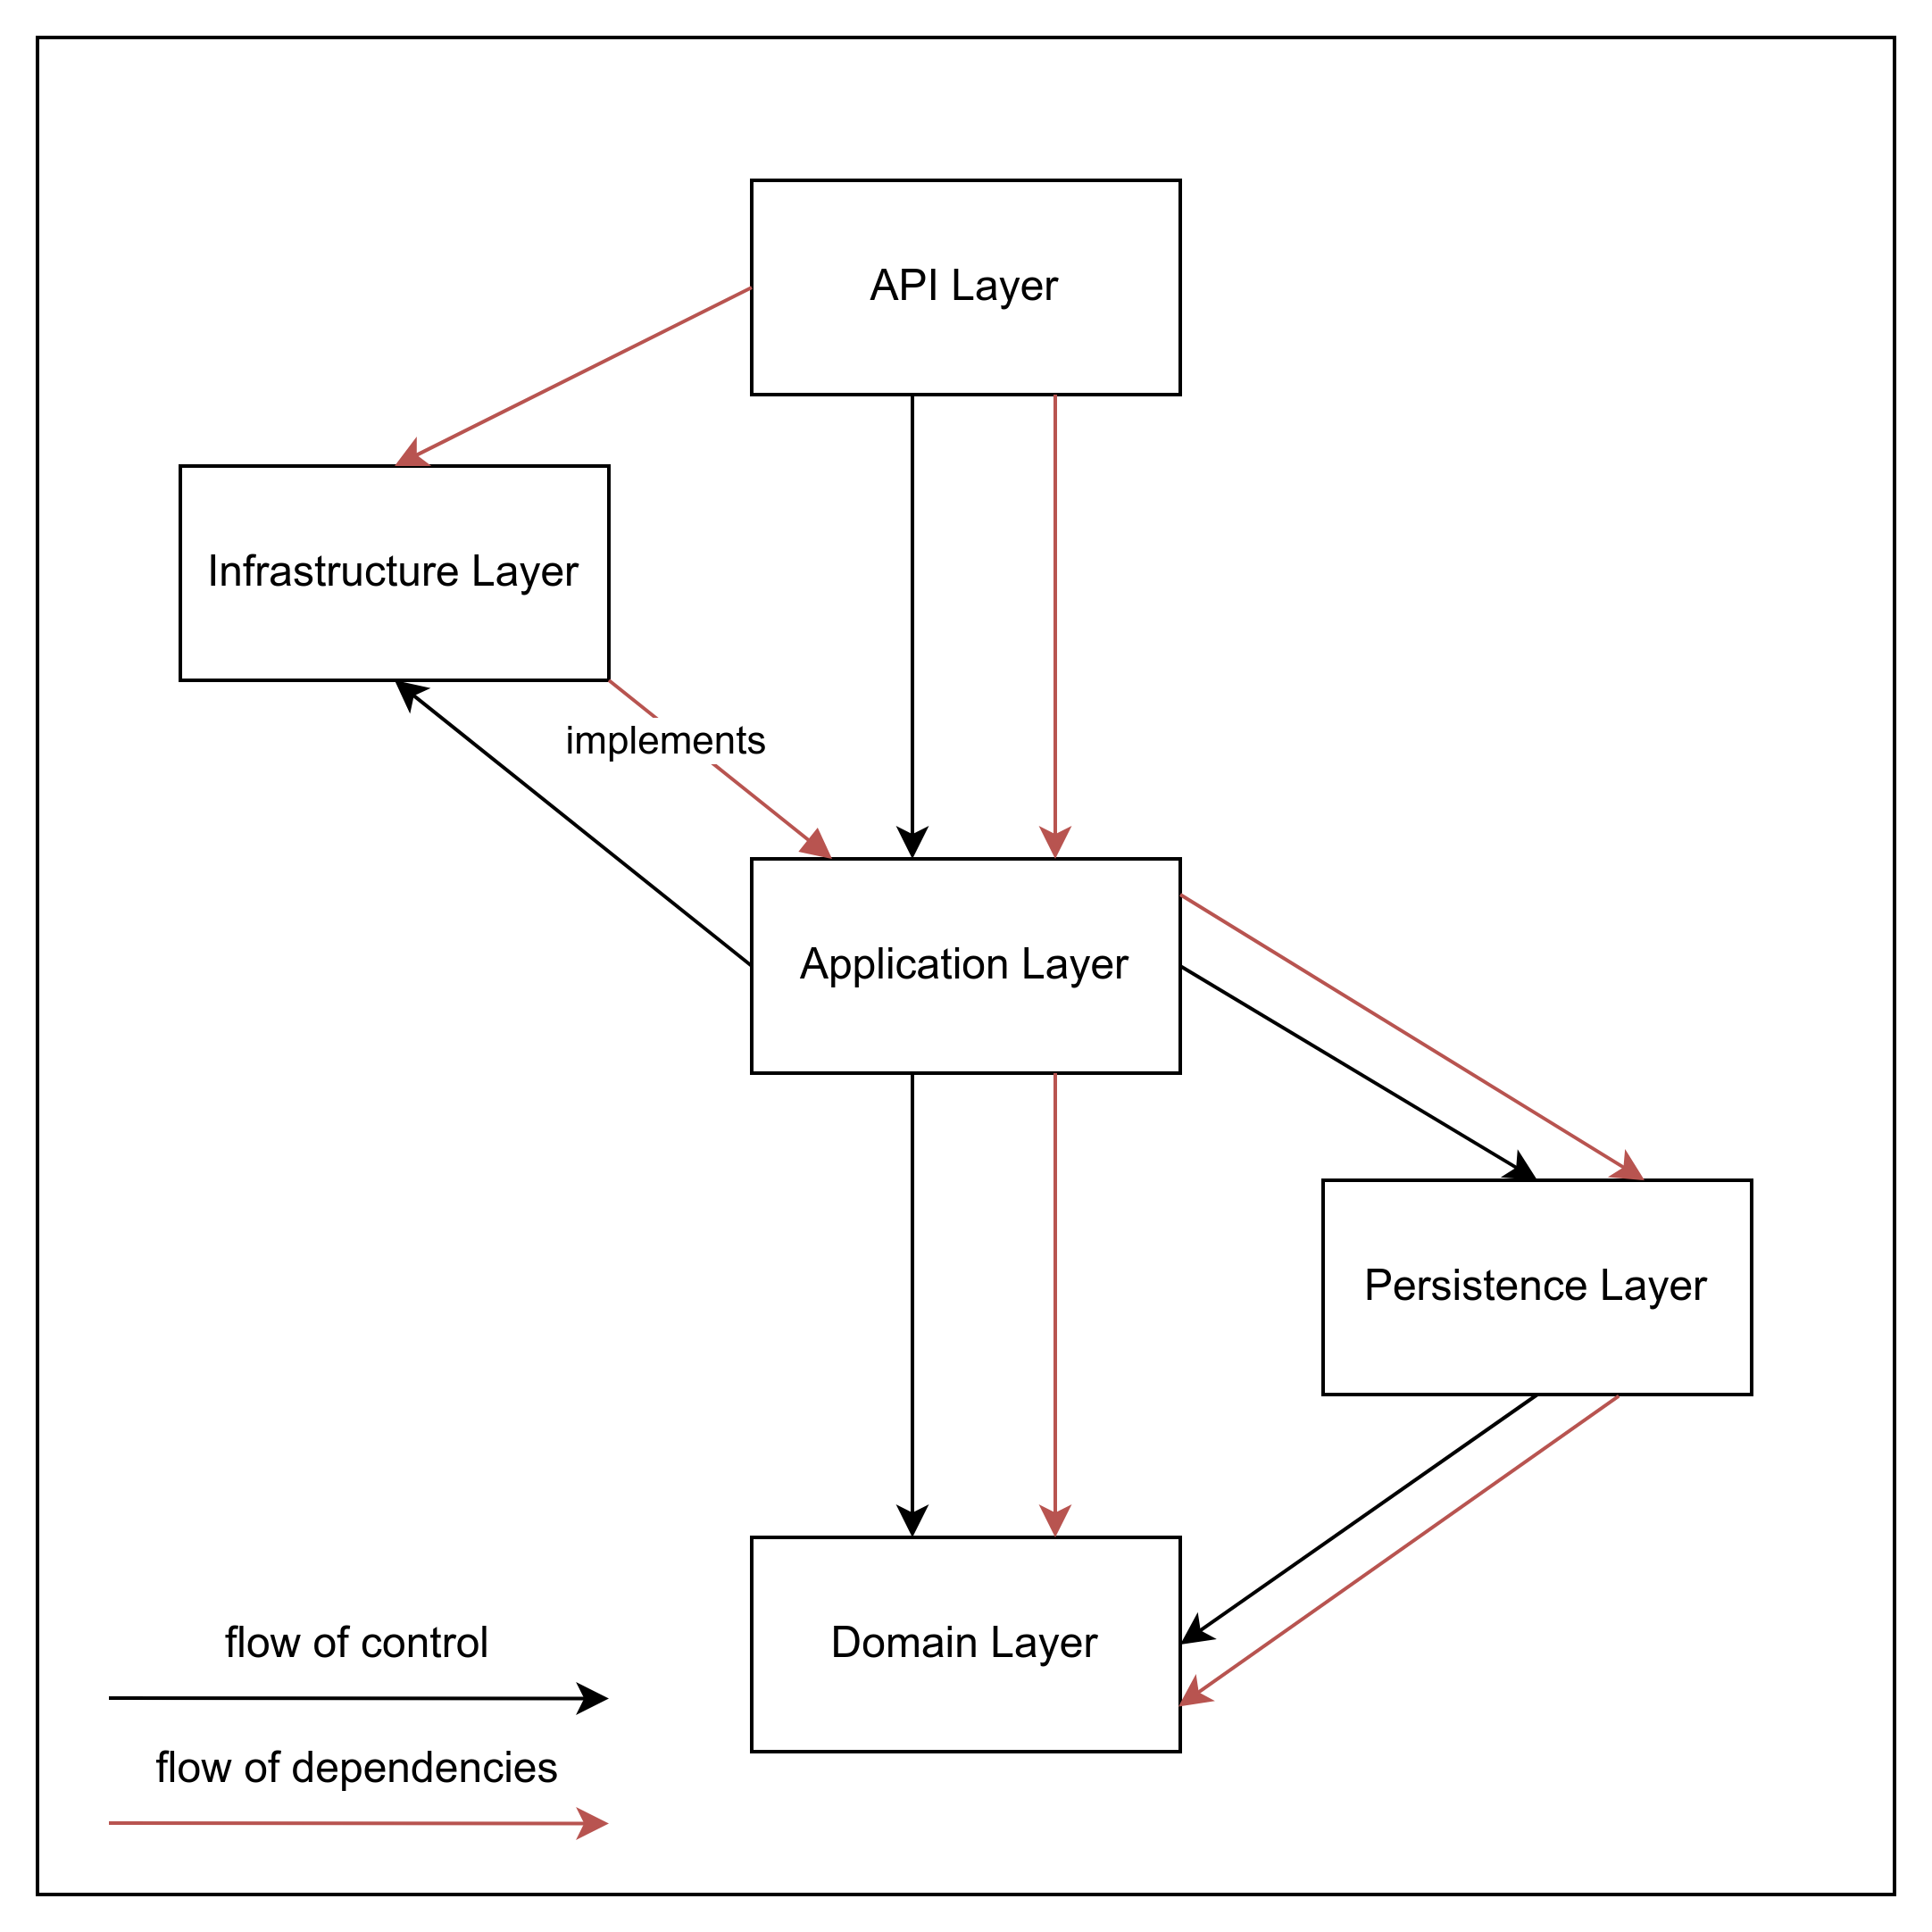
\includegraphics[width=0.96\linewidth]{backend-layers-with-flow-of-control.png}
    \caption{Backend layers}
    \label{fig:enter-label}
\end{figure}

\clearpage % https://www.overleaf.com/learn/latex/Questions/How_can_I_get_my_table_or_figure_to_stay_where_they_are%2C_instead_of_going_to_the_next_page%3F

\subsection{Diagrams}

\subsubsection{Domain class diagram}

\begin{figure}[!ht]
    \centering
    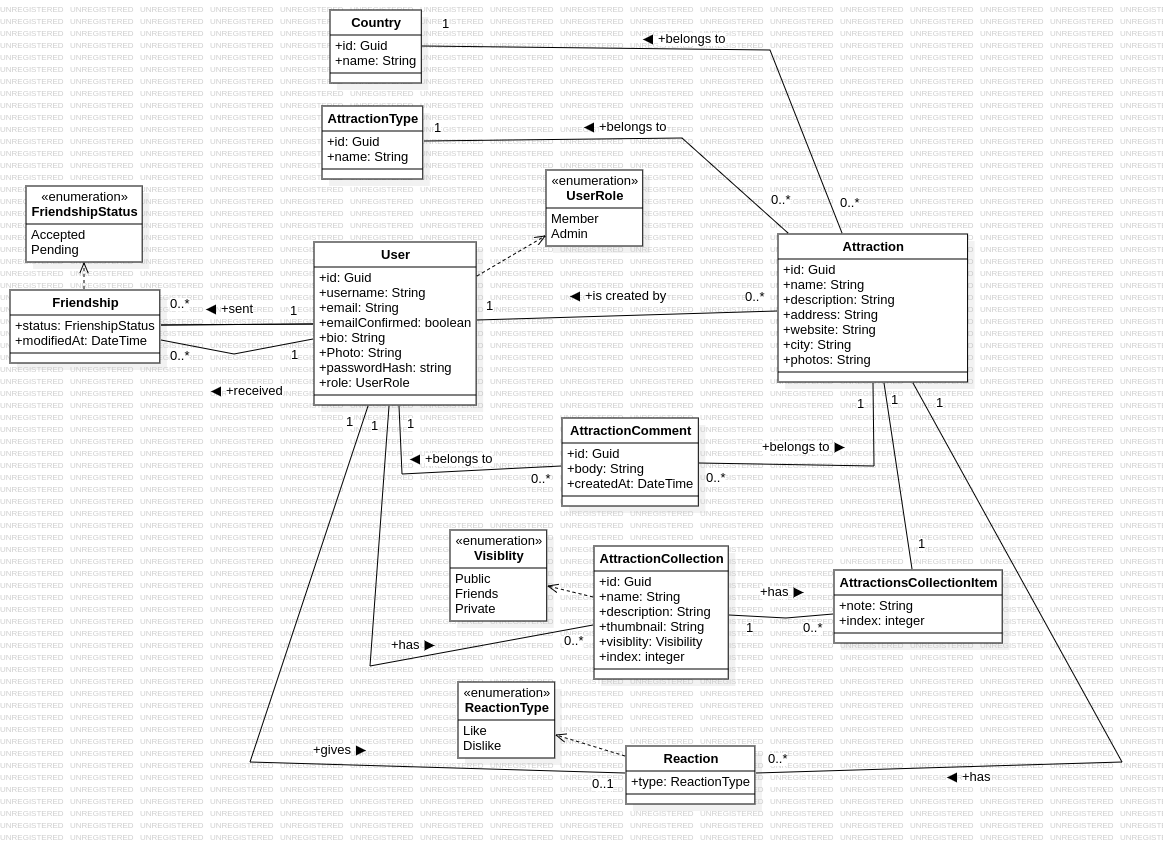
\includegraphics[width=1\linewidth]{domain-class-diagram.png}
    \caption{Domain class diagram (*associations should be aggregations)}
    \label{fig:enter-label}
\end{figure}

\subsubsection{Database diagram}

\par Since the database is generated by the Entity Framework, its structure is similar to the domain:

\clearpage % https://www.overleaf.com/learn/latex/Questions/How_can_I_get_my_table_or_figure_to_stay_where_they_are%2C_instead_of_going_to_the_next_page%3F

\begin{figure}[!ht]
    \centering
    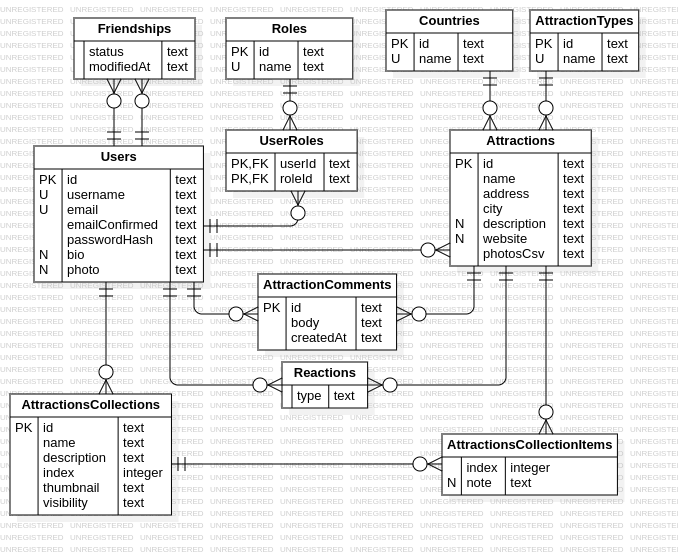
\includegraphics[width=0.7\linewidth]{db-diagram.png}
    \caption{Database diagram}
    \label{fig:enter-label}
\end{figure}


\subsubsection{Business logic class diagram}

\begin{figure}[!ht]
    \centering
    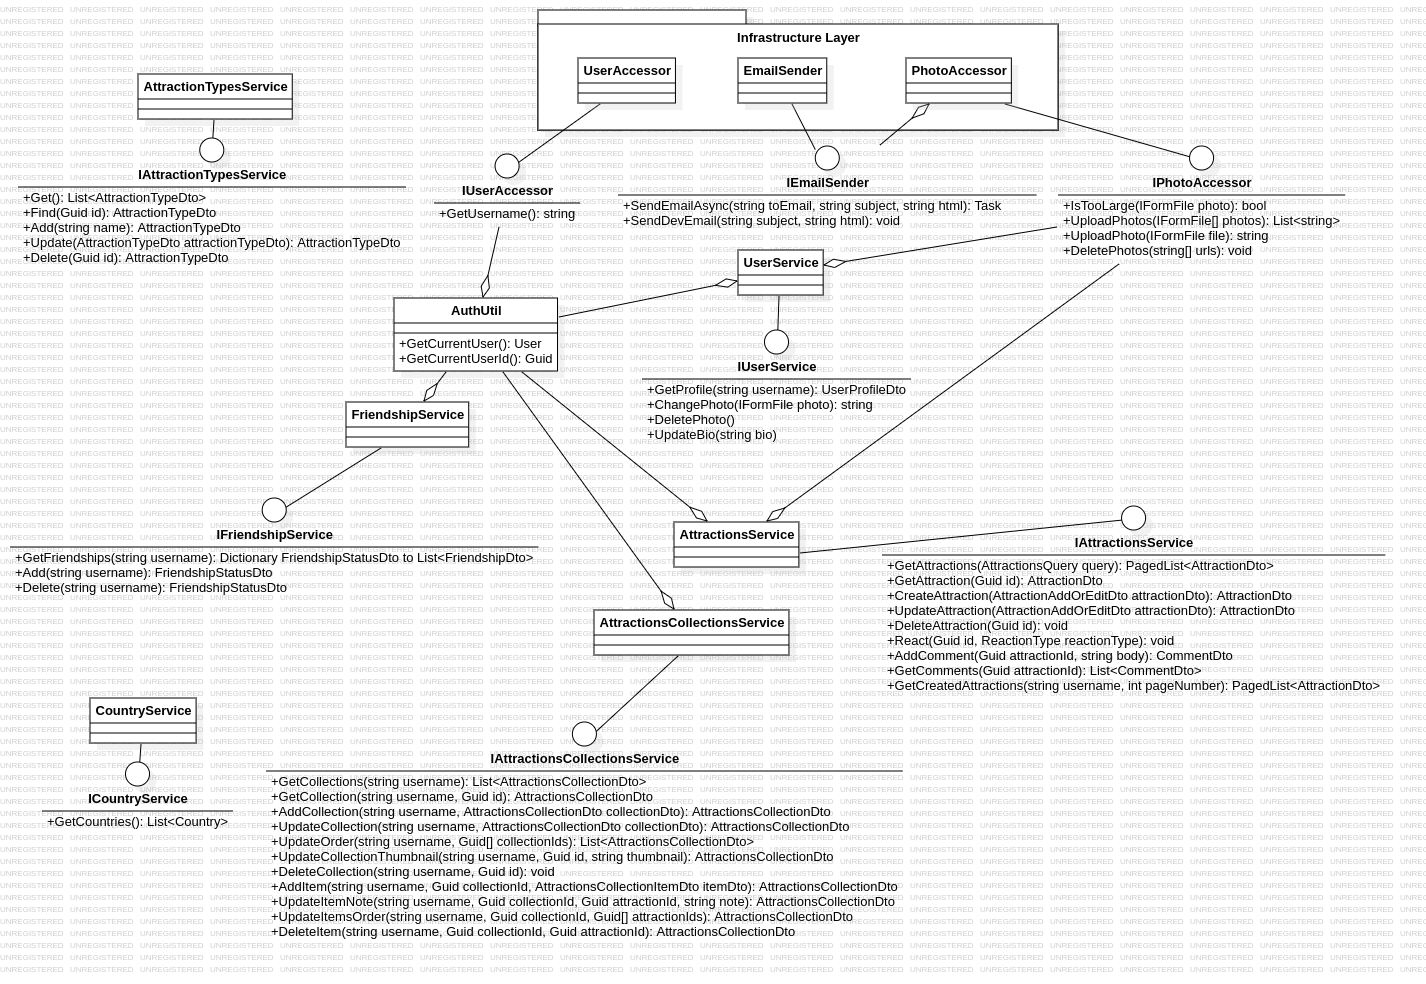
\includegraphics[width=1\linewidth]{business-class-diagram.png}
    \caption{Business logic class diagram}
    \label{fig:enter-label}
\end{figure}

\begin{figure}
    \centering
    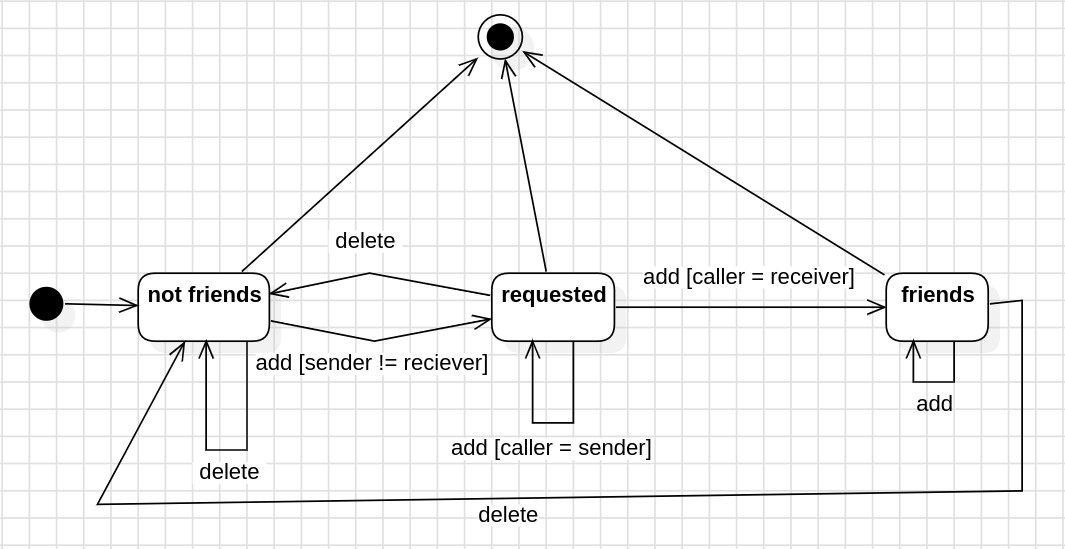
\includegraphics[width=1\linewidth]{friendship-statechartdiagram.png}
    \caption{Friendship statechart diagram}
    \label{fig:enter-label}
\end{figure}

\begin{figure}
    \centering
    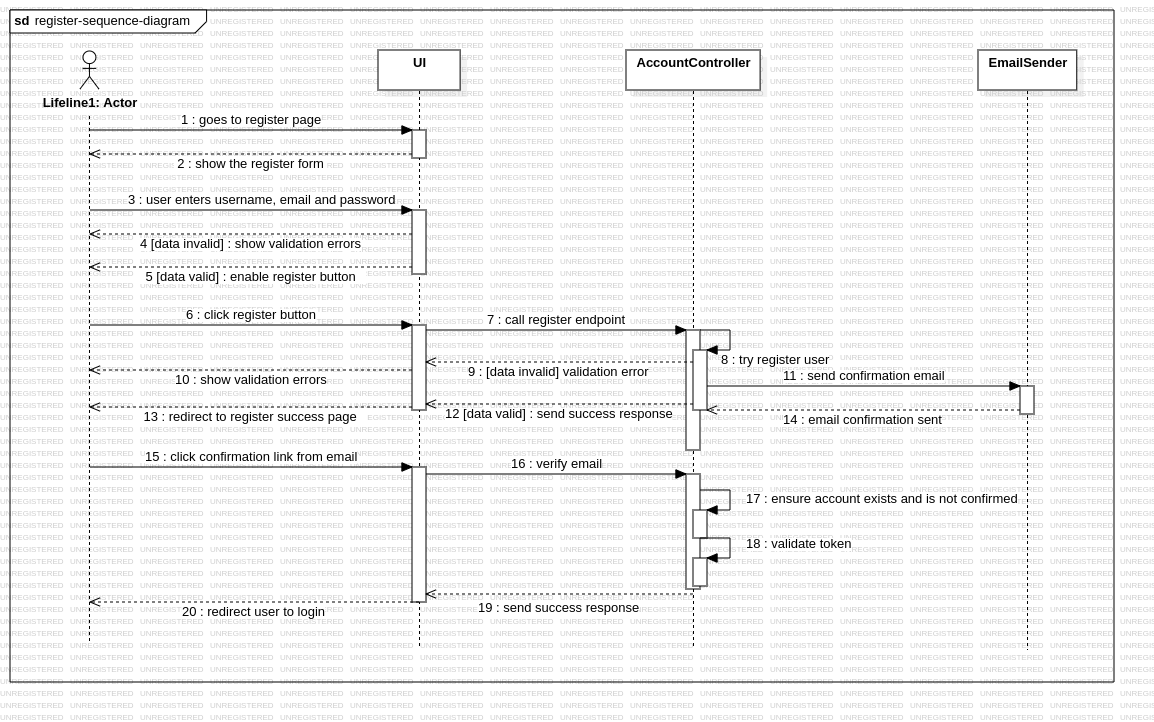
\includegraphics[width=1\linewidth]{register-sequence-diagram.png}
    \caption{Register sequence diagram}
    \label{fig:enter-label}
\end{figure}

\section{Implementation}

\subsection{ORM Mapping}

\par Entity Framework was used to map the domain classes to the database tables. In order to achieve that, the domain classes have to be used as type parameters for properties of type \textit{DbSet} inside a class that inherits from the framework's class \textit{DbContext}. In this case the class is \textit{IdentityDbContext} because it offers user management features and it is also a descendant of the \textit{DbContext} class. This \textit{IdentityDbContext} class takes as type parameters a class used for mapping the user, a class used for mapping the user role and the type of the primary key used for those two.

\begin{figure}[!ht]
    \centering
    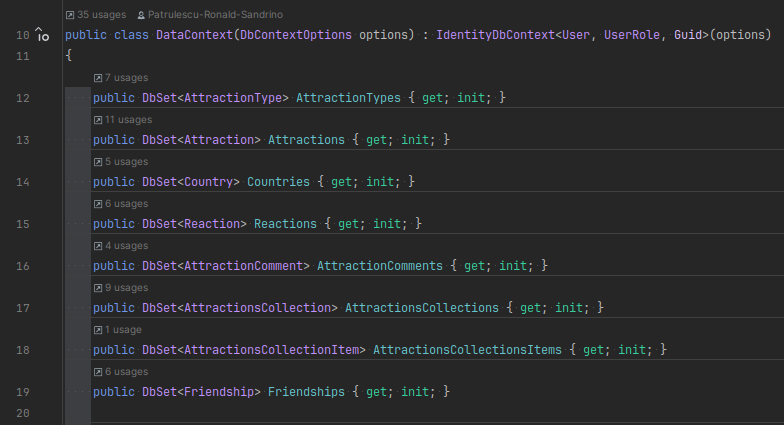
\includegraphics[width=1\linewidth]{4.3.1_dataContext.png}
    \caption{\textit{DataContext} class' properties}
    \label{fig:enter-label}
\end{figure}

\par The to be generated tables can be further configured by overriding the \textit{OnModelCreating} method of the \textit{DataContext} class. There you can define more complex primary keys, foreign keys, delete behaviors, unique indexes, check constraints, conversions, etc.

\clearpage % https://www.overleaf.com/learn/latex/Questions/How_can_I_get_my_table_or_figure_to_stay_where_they_are%2C_instead_of_going_to_the_next_page%3F

\begin{figure}[!ht]
    \centering
    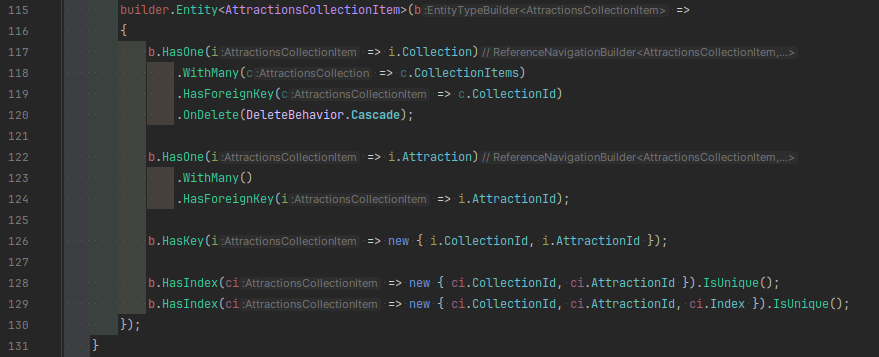
\includegraphics[width=0.95\linewidth]{4.3.1_sample-of-OnModelCreating.png}
    \caption{Example of configuring the database tables generation by overriding the \textit{OnModelCreating} method}
    \label{fig:enter-label}
\end{figure}

\par Furthermore, the defined \textit{DataContext} class has to be registered to the application services by using the \textit{AddDbContext} method. This also registers it for dependency injection so it can be used inside the service classes. This is also where the database provider is set up, which requires a method for registering it (which is usually provided by the package used for the database provider), \textit{UseSqlite} in this case, and a connection string.

\begin{figure}[!ht]
    \centering
    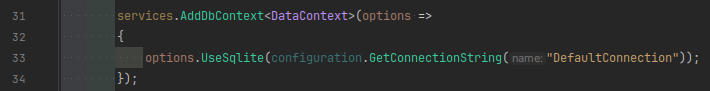
\includegraphics[width=1\linewidth]{4.3.1_AddDbContext.png}
    \caption{Registering the \textbf{DataContext} class}
    \label{fig:enter-label}
\end{figure}


\subsection{Automapper}

\par Automapper is an object-object mapper. It is used in this app in order to do conversions between domain classes and DTO classes. Mappings can be configured using profiles, which are classes that inherit from Automapper's Profile class. The profile is then registered to the DI container of application services:

\begin{figure}[!ht]
    \centering
    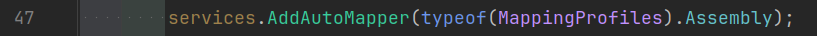
\includegraphics[width=1\linewidth]{4.3.2_automapper-injection.png}
    \caption{Registering Automapper to the application's DI container}
    \label{fig:automapper-injection}
\end{figure}

\clearpage % https://www.overleaf.com/learn/latex/Questions/How_can_I_get_my_table_or_figure_to_stay_where_they_are%2C_instead_of_going_to_the_next_page%3F

\par Mapping for fields with the same name happens implicitly. For the rest of them, we can define custom mappings or even ignore them, as seen in Figure \ref{fig:automapper-profile}, at lines 15 and 21 respectively.

\begin{figure}[!ht]
        \centering
        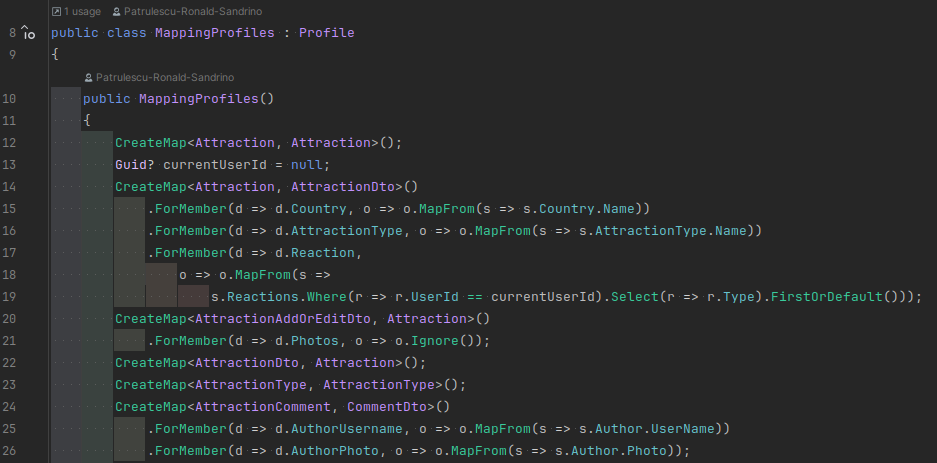
\includegraphics[width=1\linewidth]{4.3.2_automapper-profile.png}
        \caption{Example of Automapper profile configuration}
        \label{fig:automapper-profile}
\end{figure}

\begin{figure}[!ht]
    \centering
    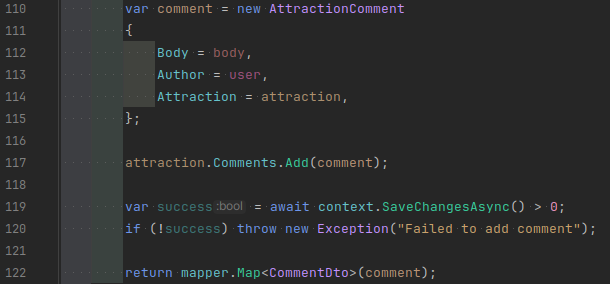
\includegraphics[width=1\linewidth]{4.3.2_automapper-usage.png}
    \caption{Example of Automapper usage (line 122)}
    \label{fig:automapper-usage}
\end{figure}


\subsection{Reading from and writing to the database}

\par Reading is done by directly accessing the \textit{DbSet} properties of the \textit{DataContext} class. For example, in Figure \ref{fig:database-read} at line 58 the contents of table of attraction types are accessed by the AttractionTypes property on the variable context, which is an instance of \textit{DataContext} injected into the service. The contents can be further processed on the database side by using non-terminal operations, methods that return an instance of \textit{IQueryable}, like Where, Include (which does join) and \textit{ProjectTo}. Then, when awaiting the call to \textit{ToListAsync} the processed query is performed on the database.

\begin{figure}[!ht]
    \centering
    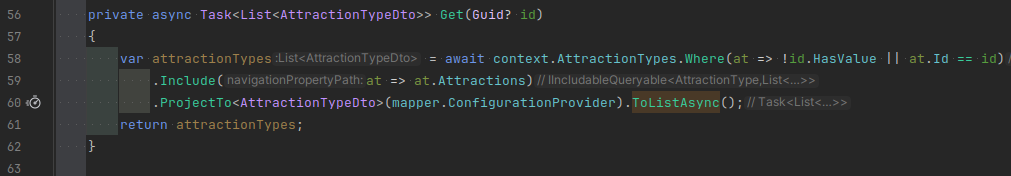
\includegraphics[width=1\linewidth]{4.3.3_database-read.png}
    \caption{Reading from the database}
    \label{fig:database-read}
\end{figure}

\par Writing to the database is done in 2 steps: 1. calling \textit{Add}/\textit{Remove} (and derivatives like \textit{AddAsync} or \textit{RemoveRange}) on either the \textit{DbSet} property or the DataContext instance, or by directly updating a domain class instance managed by the DataContext and which comes from a read operation and 2. by calling \textit{SaveChanges} on the \textit{DataContext} instances. An add example can be seen in Figure \ref{fig:automapper-usage} and an update example can be seen in Figure \ref{fig:database-write-update}

\begin{figure}[!ht]
    \centering
    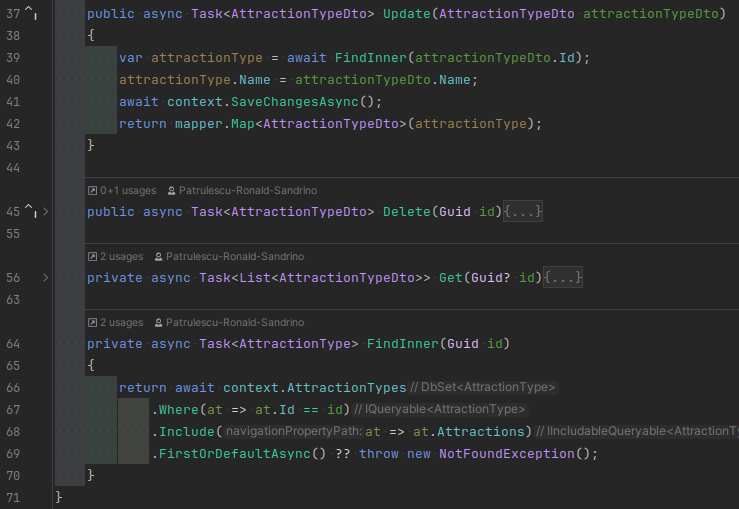
\includegraphics[width=1\linewidth]{4.3.3_database-write-update.png}
    \caption{Example of database update operation}
    \label{fig:database-write-update}
\end{figure}

\subsection{URL Mapping}

\par Each URL path is prefixed by the name of the controller. This is achieved by having all the controllers inherit from BaseApiController, which defines the path prefix using the Route annotation (Figure \ref{fig:url-mapping-baseapicontroller}). The rest of the URL path is defined by the argument of the annotations used for declaring the HTTP methods used (Figure \ref{fig:url-mapping-endpoints}). It can be observed that the paths can be parameterized.

\begin{figure}[!ht]
    \centering
    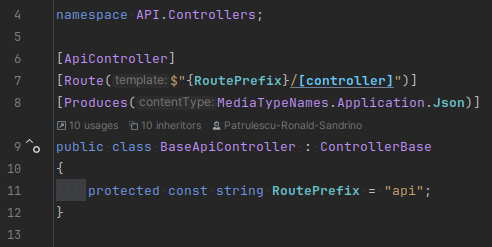
\includegraphics[width=1\linewidth]{4.3.4_url-mapping-baseapicontroller.png}
    \caption{How the name of the controller is added to the URL}
    \label{fig:url-mapping-baseapicontroller}
\end{figure}

\begin{figure}[!ht]
    \centering
    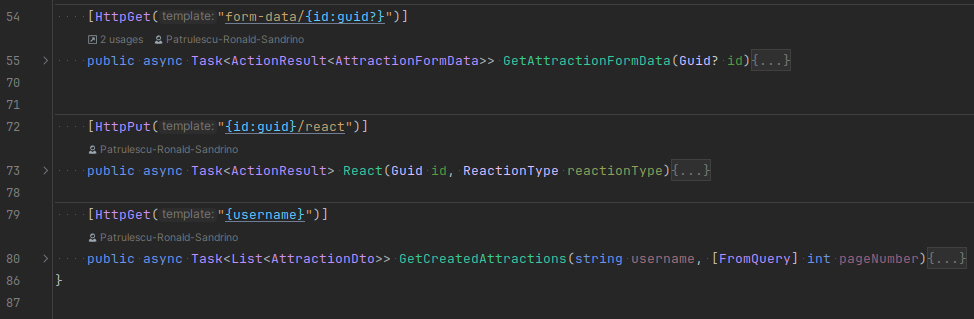
\includegraphics[width=1\linewidth]{4.3.4_url-mapping-endpoints.png}
    \caption{Defining endpoints}
    \label{fig:url-mapping-endpoints}
\end{figure}

\subsection{Dependency Injection}

\par Dependency injection is achieved by specifying the needed classes as constructor parameters (\ref{fig:dependency-injection_usage}) and then registering those classes when the application is created (\ref{fig:dependency-injection_registering}). Here, they are registered using the \textit{AddScoped} method, which registers their lifetime per HTTP request.


\begin{figure}[!ht]
    \centering
    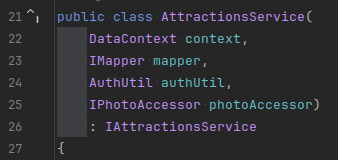
\includegraphics[width=0.5\linewidth]{dependency-injection_usage.png}
    \caption{Injection of dependencies using the primary constructor}
    \label{fig:dependency-injection_usage}
\end{figure}

\begin{figure}
    \centering
    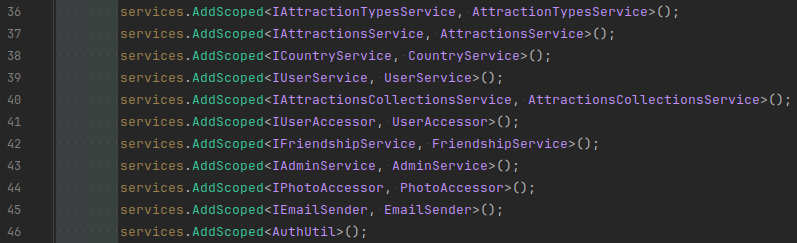
\includegraphics[width=1\linewidth]{dependency-injection_registering.png}
    \caption{Registration of dependencies}
    \label{fig:dependency-injection_registering}
\end{figure}

\subsection{Error handling}

\par When the Web API is created (in the entry point of the application - the \textit{Program.cs} file) there are 2 things that are done. The first one is the registration of the services (Figure \ref{fig:exception-handling_registration} lines 18 - 28) and the second is the configuration of the HTTP request pipeline (Figure \ref{fig:exception-handling_registration} lines 33 - ...). The order in which the middlewares are configured is the order in which they are run. And, the reason the exception handling middleware is the  first in the pipeline (Figure \ref{fig:exception-handling_registration} line 33) is to catch any exception that occurs later in the pipeline. The purpose of the exception middleware is to have a single piece of code that handles what response is given, depending on the exception, to the initiator of the HTTP request. In this application, it changes the status code depending on the exception (Figure \ref{fig:exception-handling_middleware} lines 24 - 33), writes the validation errors to the body of the response (Figure \ref{fig:exception-handling_middleware}) line  33) and adds the stacktrace to the response only if the app is running in development mode.

\begin{figure}
    \centering
    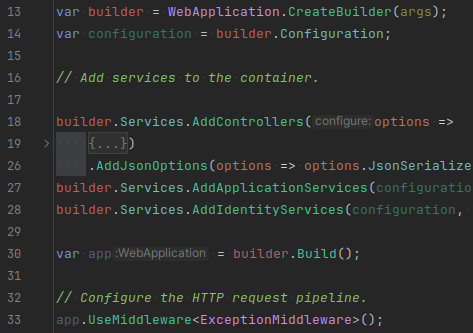
\includegraphics[width=1\linewidth]{exception-handling_registration.png}
    \caption{Registration of the exception handling middleware}
    \label{fig:exception-handling_registration}
\end{figure}

\begin{figure}
    \centering
    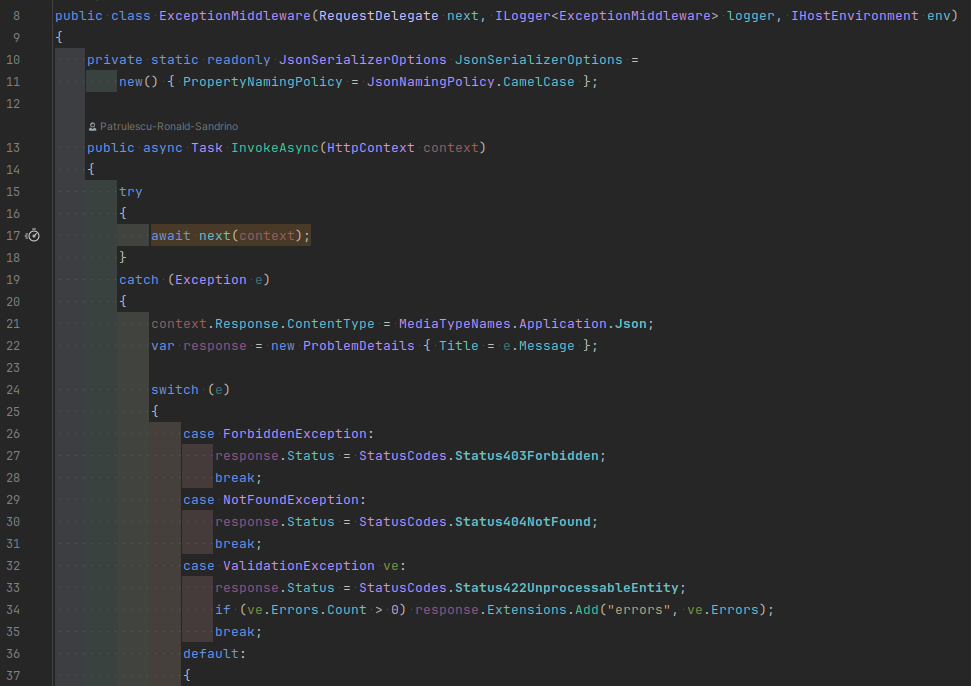
\includegraphics[width=1\linewidth]{exception-handling_middleware.png}
    \caption{Middleware for exception handling}
    \label{fig:exception-handling_middleware}
\end{figure}

\chapter{Conclusions and future work}
%\chapter*{Concluzii}
\label{conclusions}

\section{Conclusions}
\par ASP.NET Core offers a reliable and easy choice for Web API application development. To further solidify this, the minimal API that can be created is a 4-lines long code (Figure \ref{fig:conclusions_minimal-web-api}). And, by adding the Entity Framework into the mix to take care of the database side, all that remains is the business logic.

\begin{figure}[!ht]
    \centering
    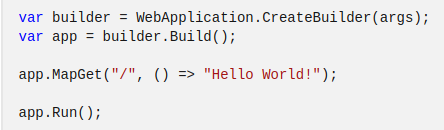
\includegraphics[width=1\linewidth]{conclusions_minimal-web-api.png}
    \caption{Minimal API with ASP.NET Core \cite{microsoftMinimalApi}}
    \label{fig:conclusions_minimal-web-api}
\end{figure}

Since React is an unopinionated library, it leaves room for a high degree of customization. But that is not without cost, since it could lead to having to reinvent the wheel and/or ending up with tons of dependencies. It's like the space-time trade-off, the best choice depends on the individuality of each project.

\section{Future work}

\subsection{Internationalization (i18n) and localization (l10n)} 

\par Internationalization (i18n) is the provisioning of the application with different languages. Internationalizing the application can expand its the reach to a global audience. Besides, since attractions could be all over the world, having the ability to switch between languages creates an easy way for comparison, which is handy for language learners.

\par Localization is the adaptation of the application to specific locales. Specifically, referring to date and time formats; number formats; symbols, icons, and colors; Right-to-Left (RTL) Language Support. This too increases the regional reach of the application.

\subsection{Accessibility (A11y)}

\par Accessibility means making the web application usable by as many people as possible, including those with disabilities. This increases the potential user base of the application.

\subsection{Responsive Design} 

\par This means making the app usable on various devices, like phones, tablets and even smart TVs. Currently the app is the design for PC/laptop screen sizes only. 

\subsection{Animations}

\par Adding animations to the application will improve the smoothness of the application and the user experience.

\subsection{Visibility for attractions}

\par Currently, only attractions collections allow setting the visibility. By extending it to attractions, it can improve the user experience by increasing the user's control of what parts of their information is publicly available. And, you can even extend the app's scope beyond the standard meaning of attractions. For example you could add your secret favorite place, even if it's not what you would normally call an attraction.

\subsection{Shared collections}

\par Are you planning a multi-destination trip with your friends/family and want to put all the suggestions or even the final itinerary in one shared place? That's where shared collections would come in.

\subsection{Personalized recommendations}
\par All the user interactions produce data: what attractions the user interacts with and how much time they spend on those attractions? what about their friends? is there a pattern to all the collections they made or to the attractions they created? etc. With collected data on such questions, an algorithm could be made that would give personalized recommendations to the users. 

\subsection{Abstracting the usage of the the UI design library}
\par Unlike the other ideas, which have in mind the user experience (UX), this is about the developer experience. The UI design library in this application (Material UI) is used as is, by directly using the components provided. But those components could be abstracted into other components, put together in one place, that only expose functionality and no implementation details of the design library. This way, should a need for the change of the UI design library appear, the required work to achieve that would be way more tedious.


\subsection{Legal and informational pages}
 \par Pages like Terms and Conditions, Privacy Policy, and Contact are crucial for regulatory compliance and for for establishing trust and transparency with users.

%\addcontentsline{toc}{chapter}{Concluzii}
%\addcontentsline{toc}{chapter}{Conclusions}

\bibliography{references}

\end{document}
